\section{Modelo GRAND}

No modelo GRAND são tratados três aspectos do gerenciamento de dados: transferência automática dos dados de entrada para o local onde o arquivo será necessário; o envio de resultados é controlado evitando congestionamento da rede; priorização de localidade no disparo de tarefas para não haver transferências desnecessárias de dados degradando o desempenho. Através de uma hierarquia de gerenciadores (Figura 1) é feito o disparo e controle das aplicações. o \emph{Application Manager} (AP) recebe uma submissão de aplicação através de um usuário, os APs mandam os \emph{Submission Managers} (SM) descrições de tarefas assim, sob demanda, são instanciados os \emph{Task Managers} (TM) para controlar a submissão de tarefas a escalonadores de domínios específicos da grade, esses escalonadores recebem requisições dos TMs fazendo a execução das tarefas propriamente ditas.

\begin{figure}[htb]
\begin{center}
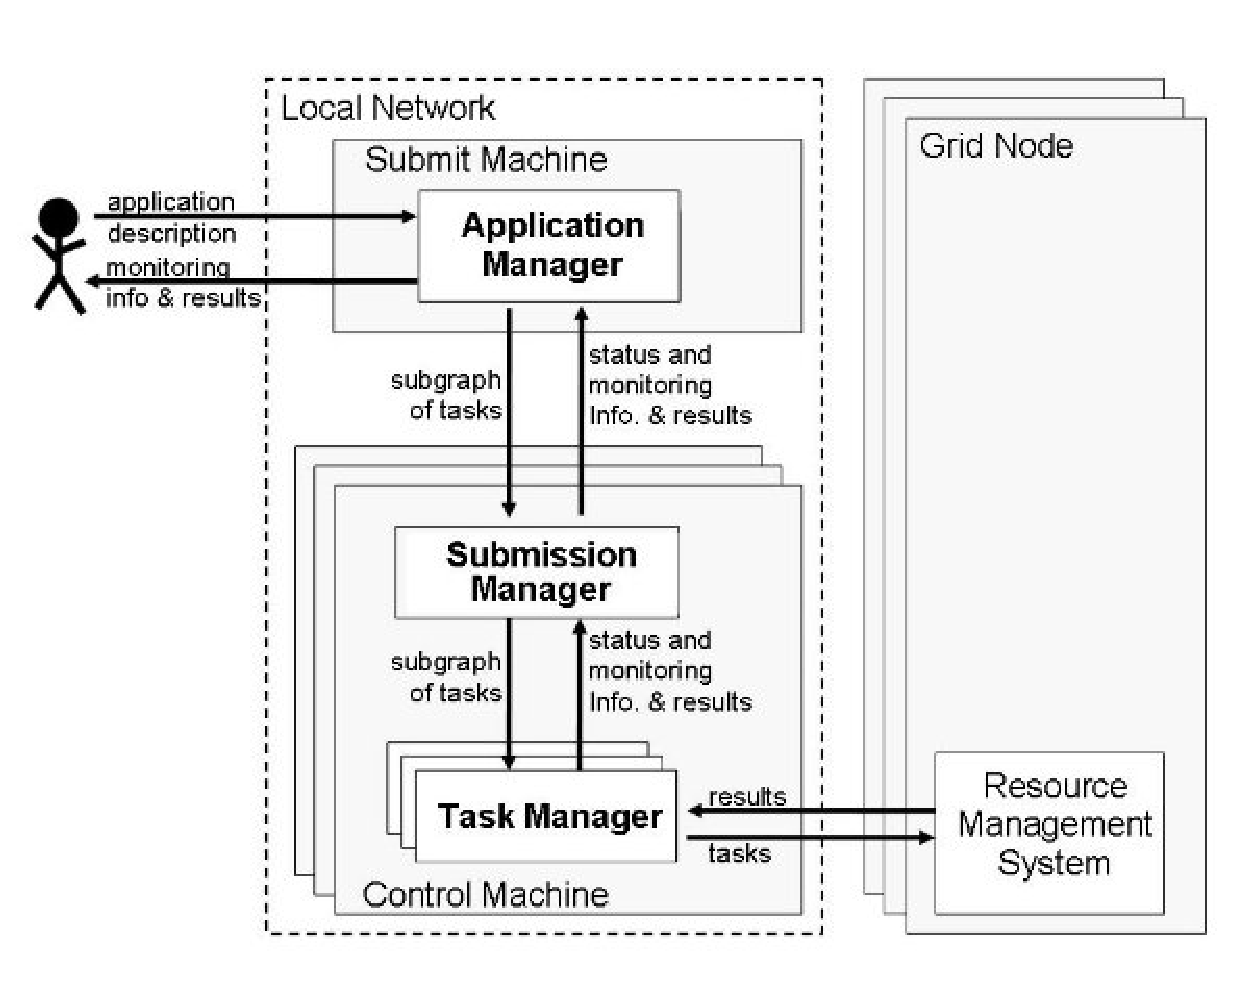
\includegraphics[scale=0.7]{./img/grand.eps}
\caption{Principais componentes do modelo hierárquico de gerenciamento de tarefas}
\label{fig:Modelo_Grand}
\end{center}
\end{figure}

%\begin{figure}[htb]
%\begin{center}
%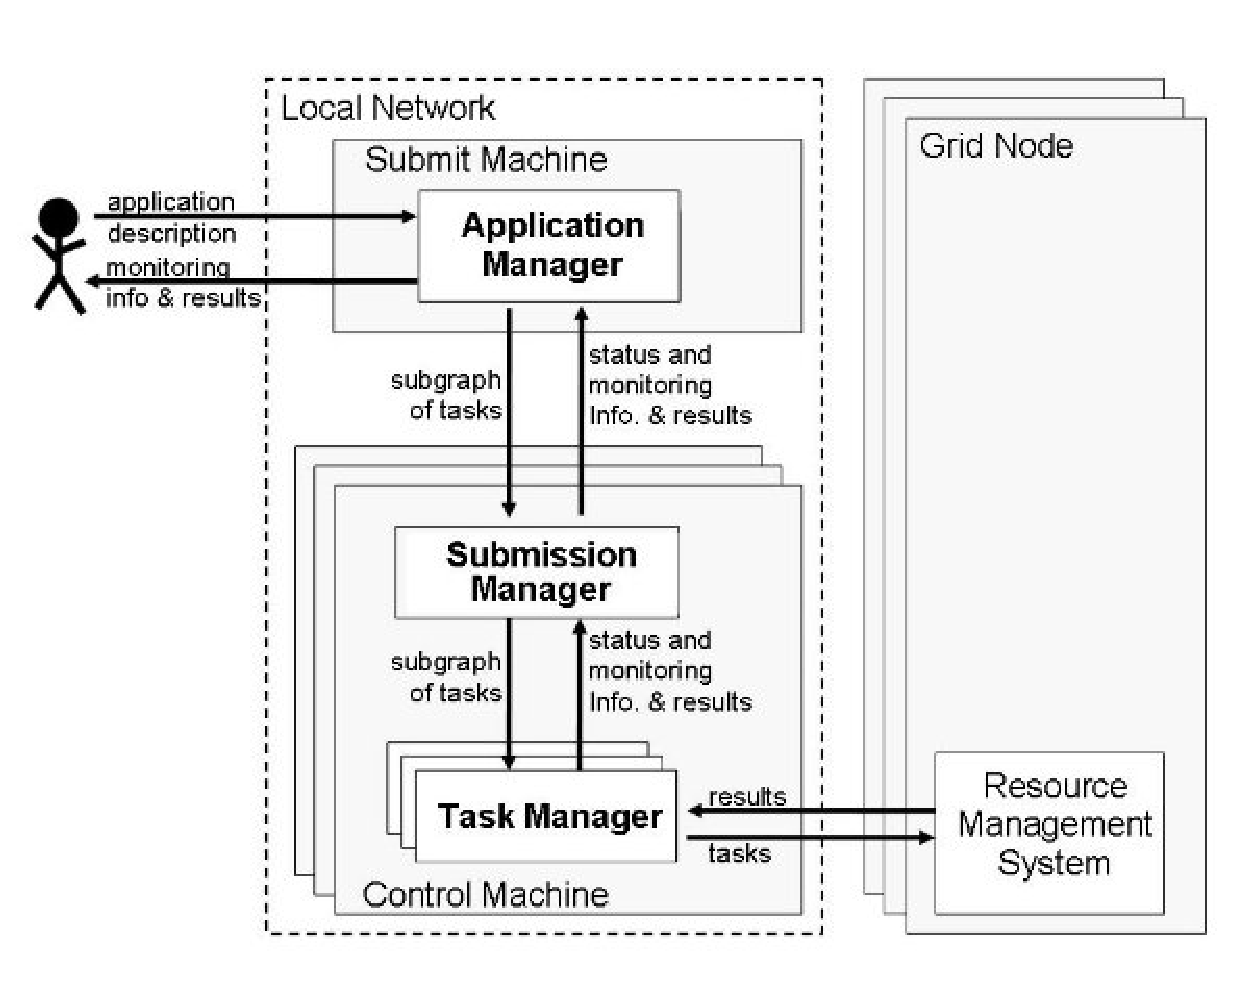
\includegraphics[scale=0.50]{./img/grand.eps}
%\caption{Principais componentes do modelo hierárquico de gerenciamento de tarefas}
%\label{fig:Modelo_Grand}
%\end{center}
%\end{figure}
